\documentclass[a4paper, titlepage, openright]{book}

\usepackage[english]{babel}
\usepackage{frontespizio}
\usepackage{amsmath}
\usepackage{amsthm}
\usepackage[linesnumbered,ruled,vlined]{algorithm2e}
\usepackage{textcomp}
\usepackage{mathtools, nccmath}
\usepackage[left=3cm,right=2cm,top=3cm,bottom=2cm]{geometry}
\usepackage{rotating}
\usepackage{subfigure}
\usepackage{url}

% force page number on page bottom part
\usepackage{fancyhdr} 
\fancyhf{}
\cfoot{\thepage}
\pagestyle{fancy}

% These Commands create the label style for tables, figures and equations.
\usepackage[labelfont={footnotesize,bf} , textfont=footnotesize]{caption}
\captionsetup{labelformat=simple, labelsep=period}
\newcommand\num{\addtocounter{equation}{1}\tag{\theequation}}
\renewcommand{\theequation}{\arabic{equation}}
\makeatletter
\renewcommand\tagform@[1]{\maketag@@@ {\ignorespaces {\footnotesize{\textbf{Equation}}} #1.\unskip \@@italiccorr }}
\makeatother
\setlength{\intextsep}{10pt}
\setlength{\abovecaptionskip}{2pt}
\setlength{\belowcaptionskip}{-10pt}

\renewcommand{\textfraction}{0.10}
\renewcommand{\topfraction}{0.85}
\renewcommand{\bottomfraction}{0.85}
\renewcommand{\floatpagefraction}{0.90}

% This styles the bibliography and citations.
\usepackage{natbib}
\setlength\bibindent{2em}
\makeatletter
\setlength{\bibsep}{0pt plus 0.3ex}

% redefine chapter -> no labeling with 1, 2, etc.
\newcommand{\mychapter}[2]{
    \setcounter{chapter}{#1}
    \setcounter{section}{0}
    \chapter*{#2}
    \addcontentsline{toc}{chapter}{#2}
}

% table of contents will contain also subsections
\setcounter{tocdepth}{2}

% change Bibliography into References
\AtBeginDocument{\renewcommand{\bibname}{References}}

% set input and output for algorithm2e
\SetKwInput{KwInput}{Input}                
\SetKwInput{KwOutput}{Output} 

\begin{document}
% -----  title page
\begin{frontespizio}
	\Universita {Verona}
	\Dipartimento {Informatica}
	\Scuola {Ph.D. in Computer Science}
	\Annoaccademico {2020--2021}
	\Titoletto {First Year Report}
	\Titolo {Predicting genetic variants effect on genomic Regulatory Elements}
	\Candidato [VR456869]{Manuel Tognon}
	\NCandidato {Student}
	\NRelatore {Supervisor}{}
	\Relatore {Prof. Rosalba Giugno}
	\NCorrelatore {Cosupervisor}{}
	\Correlatore{Prof. Luca Pinello}
\end{frontespizio}
% ------  table of contents, index of figures and tables
\tableofcontents
\listoffigures
\listoftables
% ------ Introduction
\mychapter{1}{Introduction}
Transcription Factors (TFs) are fundamental regulatory proteins playing a key role in regulating the transcriptional state, differentiation and developmental patterns of cells \citep{lambert2018human,reimold2001plasma,whyte2013master}. By binding short DNA sequences (7-20 nucleotides \citep{stewart2012transcription}) called transcription factor binding sites (TFBS) they finely regulate gene expression in a cell-specific manner. TFBS are located within gene promoters \citep{whitfield2012functional} or in distal regulatory elements, such as enhancers or silencers \citep{gotea2010homotypic,lemon2000orchestrated,nolis2009transcription}. TFs bind DNA in a sequence specific manner, recognizing similar but not identical sequences differing in few nucleotides. Often TFBS of a given TF show recurring patterns, which are referred to as \textit{motifs}. TFBS discovery or \textit{motif discovery} is one of the most studied and challenging problems in genomics and computational genomics \citep{pavesi2004silico,d2006does,zambelli2013motif}. TFBS motif discovery can be defined as the problem of finding short similar nucleotide patterns, shared by all or large fractions of sequences bound by the same TF, building the motif. TF motifs can be described and predicted by several models, such as Position Weight Matrices (PWMs) \citep{stormo2000dna}, Markov models (MMs) \citep{durbin1998biological}, or Deep Neural Networks (DNNs) \citep{talukder2021interpretation}. During the last two decades, have been introduced several experimental methods to identify and characterize TFBS \textit{in vitro} and \textit{in vivo} \citep{jolma2011methods}, such as protein binding microarray (PBM) \citep{berger2006compact,berger2009universal}, HT-SELEX \citep{jolma2010multiplexed}, ChIP on Chip \citep{pillai2015chip,collas2008chop}, or ChIP-seq \citep{johnson2007genome,mardis2007chip}. These methods provide two major advantages: (i) they do not require any prior knowledge on binding site sequence, and (ii) they produce huge datasets of thousands of sequences bound by the studied TF. However, the actual binding sites remain to be computationally discovered. Several studies showed that genetic variants can significantly impact TF-DNA binding affinity \citep{de2006regulatory,weinhold2014genome,guo2018mutation}. Genome-wide association studies (GWASs) uncovered thousands of genetic variants (SNPs) associated with complex human traits. The majority of identified SNPs are in non coding regions, often corresponding to functional regulatory elements, such as enhancers \citep{maurano2012systematic}. This suggests that gene misregulation may be mediated by SNPs modulating TF-DNA binding interactions. In fact, these variants may perturb TF-DNA binding specificity, ultimately changing downstream gene expression \citep{deplancke2016genetics}. Importantly, mutations altering TFBS can occur in haplotypes conserved within a population of individuals \citep{kasowski2010variation}, producing population specific TFBS motifs. Similarly, cell-type specific genetic variation can produce different motifs for the same TF. Therefore, developing new computational methods enabling haplotype- and variant-aware motif discovery is fundamental to describe genetic variation impact on TFBS at population level. Moreover, it is important that such models are easily interpretable by humans.
% ------ Background on Motif Discovery
\mychapter{2}{Background on Motif Discovery}
TFBS motif discovery can be defined as follows. Given a set of nucleotide sequences $S$ produced by experimental assays (\textbf{Fig.\ref{fig:md}}) sharing a common biological function, find one or more motifs, built with one or more sets of short similar patterns, appearing in a large fraction of $S$. Therefore, it is fundamental to allow for experimental errors and potential false positive in $S$. To assess motifs statistical significance, they should not appear with similar frequency in sets of background DNA sequences $B$. Moreover, patterns building the motif should not have the same degree of similarity found in $b_{i} \in B$. Motifs can be encoded and represented with different models $M$. Motif model choice and construction is fundamental. In fact, $M$ is often used to predict new potential occurrences of TFBS motifs in DNA sequences, not used during model training procedure, and potentially assess the effects of genetic variants on TF-DNA binding affinity. The various methods introduced to solve this challenge mainly differ on three points: (i) the method employed to derive the motif, (ii) the model chosen to represent the motif, and (iii) how statistical significance of motifs is assessed and which background model is used \citep{zambelli2013motif}.
\begin{figure}
	\centering
	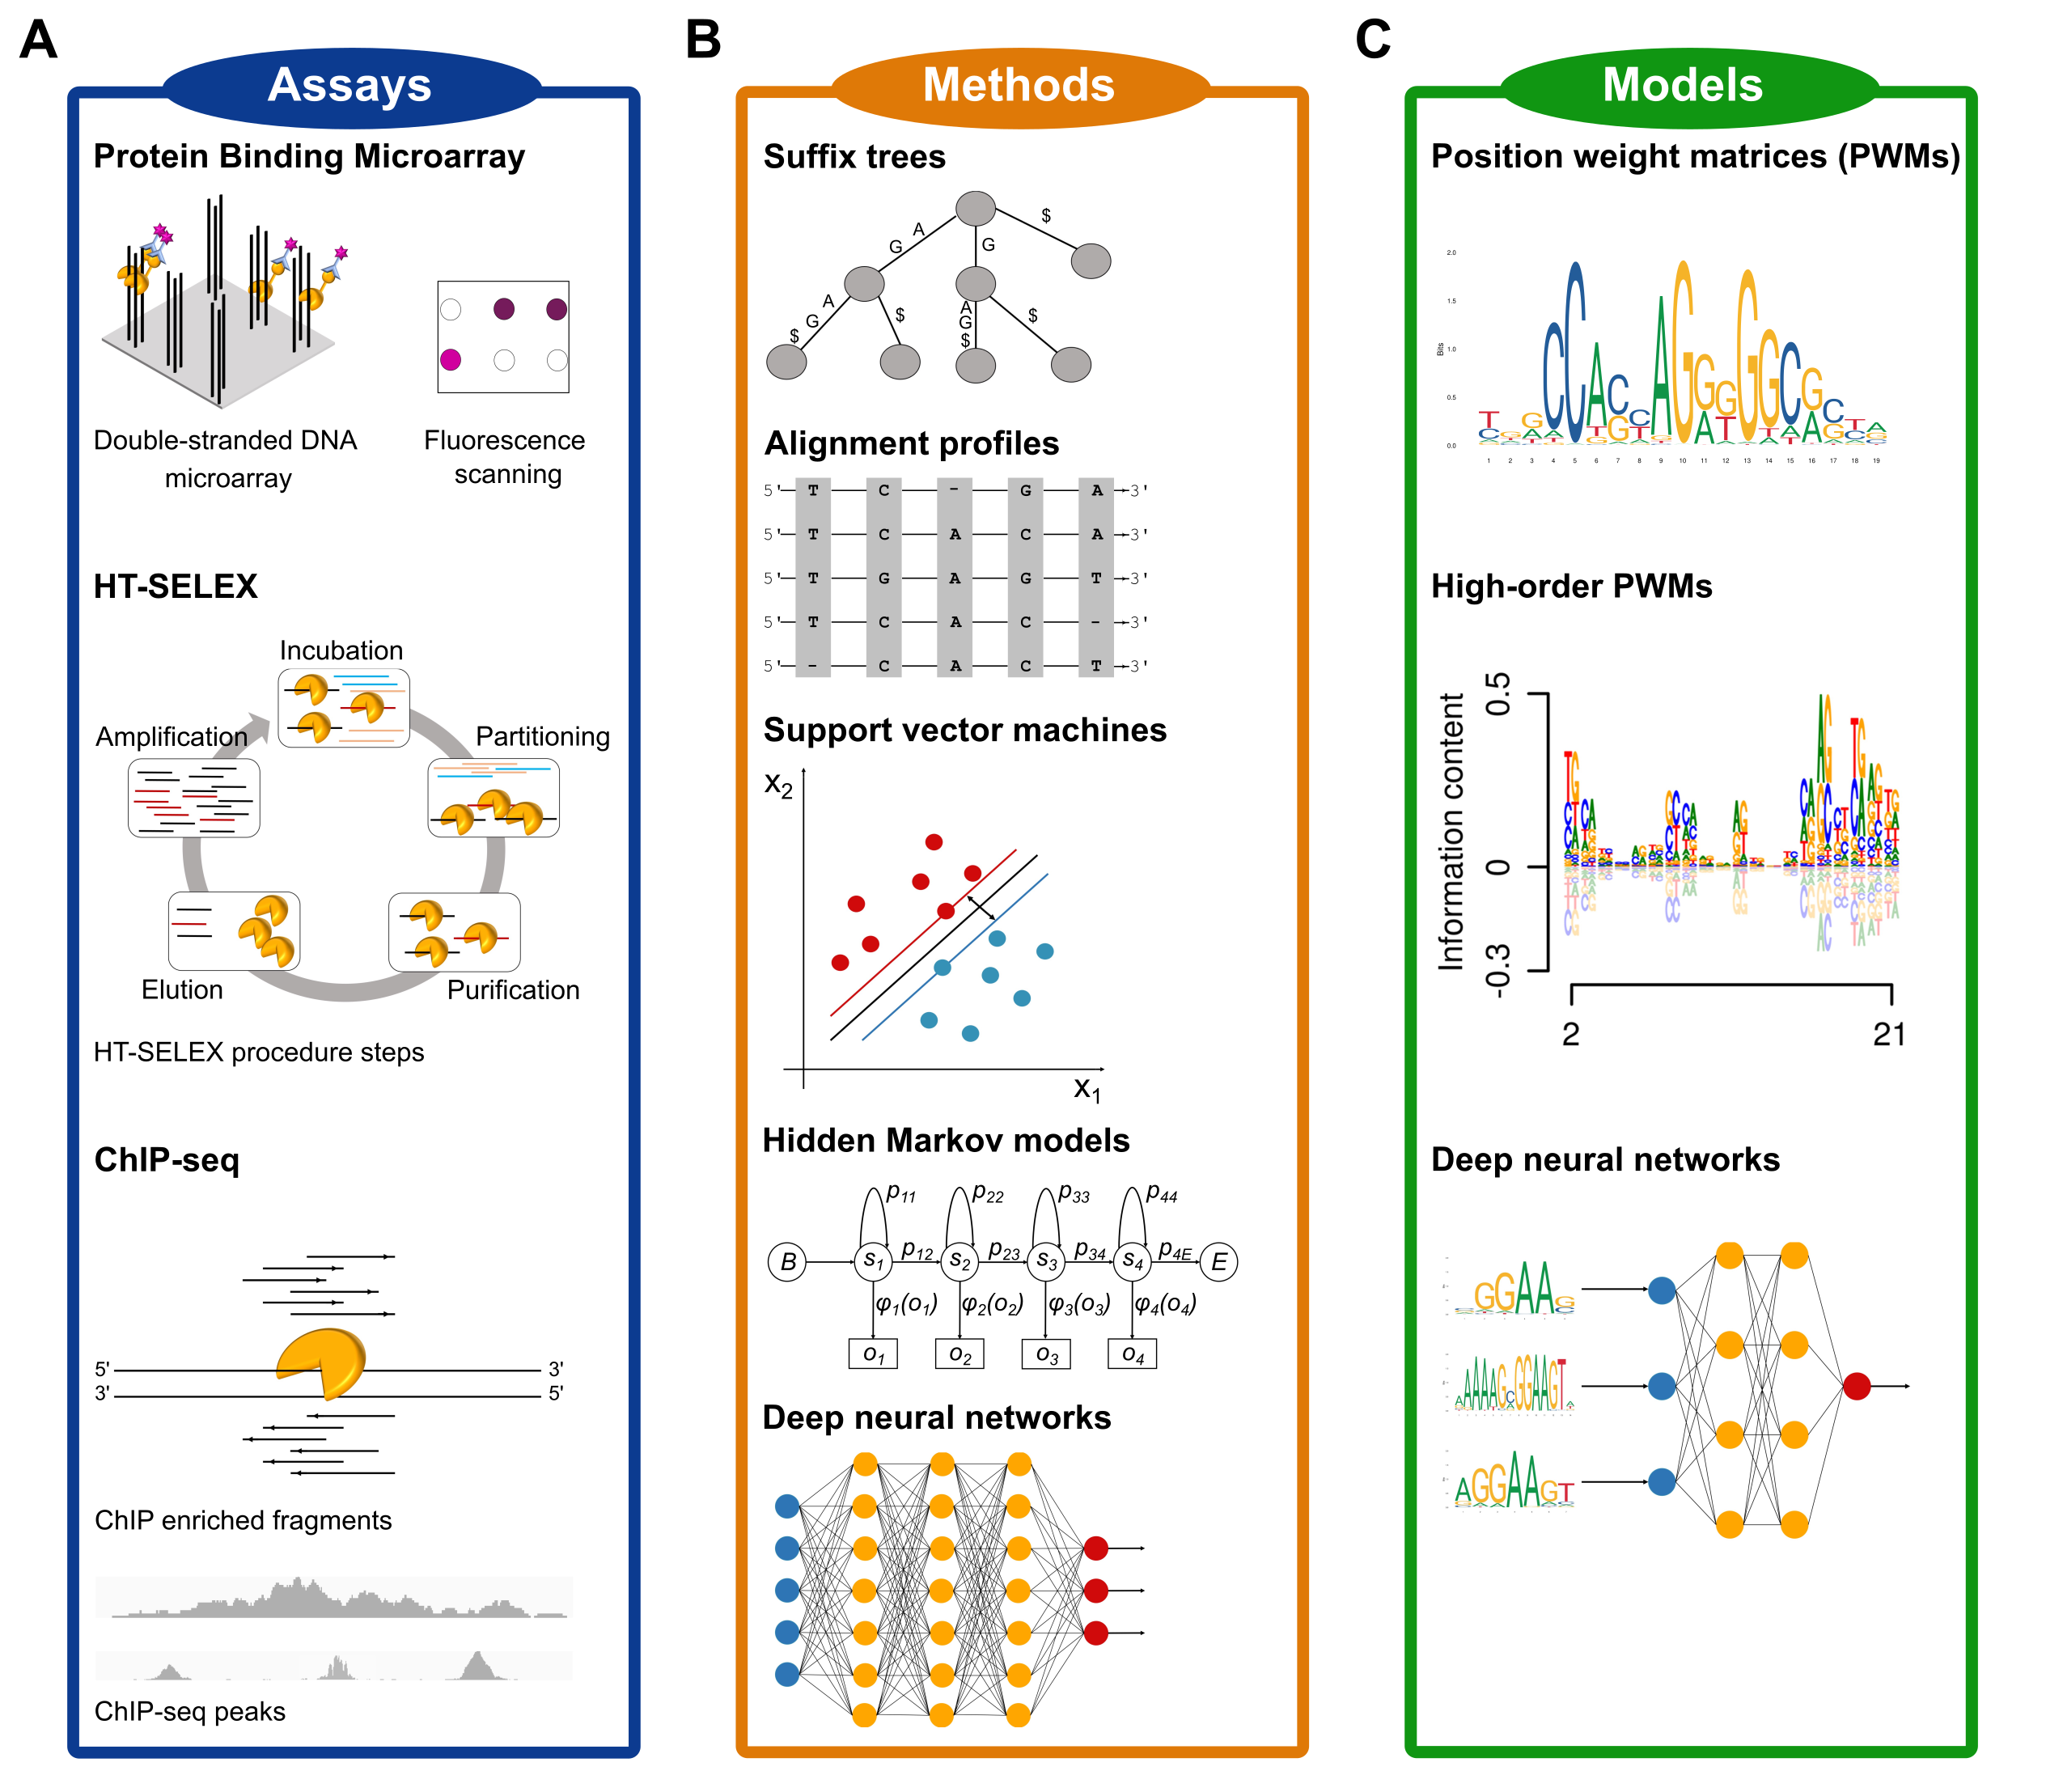
\includegraphics[width=\textwidth]{figures/Fig1.png}
	\caption[Schematic representation of motif discovery workflow.]{Schematic representation of motif discovery workflow. \textbf{(A)} Experimental assays identify and characterize nucleotide sequences containing binding sites of the studied TF. The actual binding site yet remains to be discovered and characterized. Sequences identified by experimental assays constitute the input of motif discovery algorithms. \textbf{(B)} Motif discovery methods can be divided into five major classes based on the employed algorithm: consensus sequence (suffix
trees), alignment profiles, support vector machines, markov models, deep neural networks. \textbf{(C)} TFBS motifs are described and summarized in models built using patterns identified by algorithms, such as PWM, DWM or neural networks.}
	\label{fig:md}
\end{figure} 
% ---- Motif Discovery methods
\section{Motif Discovery methods}
Motif discovery methods can be classified in five classes, based on the algorithm employed to discover putative TFBS motifs: consensus sequences, alignment profiles, markov models (MM), support vector machines (SVM), and deep neural networks (\textbf{Fig.\ref{fig:md} (B)}). Algorithms employing consensus sequence methods, collect all the approximate occurrences (with up to $e$ mismatches) of each of $4^{m}$ nucleotide sequences of length $m$ ($m$ is the motif width, $\sim10-20$ bp) in the input sequences, counting the number of matches. Therefore, the general idea is to enumerate all possible DNA oligos and count how many times they are observed in the input sequence set $S$, with respect to the background dataset $B$. The most enriched and significant motifs are reported as potential binding sites and are furtherly used to build the TFBS model. This basic approach was employed in early studies on TFBS characterization \citep{waterman1984pattern,galas1985rigorous}, although shown to be very computationally demanding. The application of indexed data structures, such as suffix trees \citep{valimaki2007compressed} made the approach feasible in real-world studies. Moreover, employing suffix trees the algorithm complexity becomes exponential in the number of $e$ mismatches allowed instead on motif width $m$ \citep{zambelli2013motif}. Weeder \citep{pavesi2001algorithm,pavesi2004weeder} and SMILE \citep{marsan2000algorithms} algorithms extended the approach by performing an exhaustive matching with no restrictions on substitution positions. While SMILE compares motif occurrences frequency with those expected in $B$, Weeder checks motif occurrences in $S$ against oligos expected frequencies in all promoter regions of the same organism of input sequence set. The selected oligos are furtherly encoded in PWMs, to describe the putative motifs.

Alignment profiles provide a more powerful and flexible description of motif binding preferences. Therefore, they have been the basic idea of choice of many motif discovery methods. The general idea is to construct an alignment profile with oligos selected from $S$ and score the resulting profile according to nucleotide conservation and with a suitable measure of significance. The problem can be formalized as a combinatorial optimization, searching for the best possible combination of fixed-length motif patterns. Therefore, the goal is to find the highest scoring profile exploring all the possible alignments of fixed-length sequences from $S$. The most naive solution would be to
exhaustively enumerate all possible alignments, but it would be too computationally demanding. To solve this challenge, alignment profile-based algorithms employ different types of heuristics and combinatorial optimizations, such as Expectation-Maximization (EM) \citep{bailey1995unsupervised}, greedy \citep{hertz1999identifying}, stochastic \citep{lawrence1993detecting}, and genetic algorithms \citep{lee2018comprehensive}. MEME algorithm \citep{bailey1994fitting,bailey1995value,bailey2006meme} explores the solution space employing an EM optimization strategy. Given a starting profile, MEME iteratively substitutes some sequences of the profile with others likely to produce better solutions. Therefore, aligned sequences are more likely to fit the profile than the remaining oligos, which should fit a background model better than the profile. However, MEME EM local search strategy can reach premature convergence in local maxima. Stochastic optimization strategies, such as Gibbs sampling, attempt to avoid this important limitation [42]. While MEME build the staring alignment profile with all fixed length sequences from $S$, stochastic algorithms build the profile choosing randomly an oligo from each $s \in S$. Then, the sequence from each $s_{i} \in S$ is removed from the profile and a likelihood score is computed for each oligo in $s_{i}$ describing how well it fits the profile, rather than a background model. The removed oligo is replaced by another sequence from $s_{i}$ with probability proportional to the computed likelihood score. The procedure is iteratively repeated until convergence is reached, or after a fixed number of iterations. It is important to notice that both local and stochastic search strategies assume the one binding site appears in each input sequence. Motif sampler [43] extended the stochastic search strategy allowing for multiple or no occurrences of a motif in input sequences. Modifications of the basic Gibbs sampling procedure were introduced in AlignACE [44] and ANN-Spec, which pairs sampling procedure with an artificial neural network [45]. GLAM algorithm [46] furtherly improved stochastic optimization, by allowing the comparison between motifs of different lengths through a simulated annealing strategy. The method was furtherly improved in GLAM2 [47] to consider gaps within motifs.




% ------  begin bibliography
\bibliography{biblio}
\bibliographystyle{natbib}





\end{document}